\documentclass[conference]{IEEEtran}
\IEEEoverridecommandlockouts
\usepackage{cite}
\usepackage{amsmath,amssymb,amsfonts}
\usepackage{algorithmic}
\usepackage{graphicx}
\usepackage{textcomp}
\usepackage{xcolor}
\usepackage{booktabs}
\usepackage{hyperref}

\hypersetup{
    colorlinks=true,
    linkcolor=blue,
    filecolor=magenta,      
    urlcolor=cyan,
}

\begin{document}

\title{Vision Transformers and Multi-Modal Foundation Models: Agricultural Pathology Diagnosis and Adversarial Robustness of Zero-Shot CLIP\\
\large Coursework Technical Report -- Neural Networks and Deep Learning (Spring 2025)}

\author{\IEEEauthorblockN{Alireza Najafi Motiei}
\IEEEauthorblockA{\textit{Department of Electrical and Computer Engineering} \\
\textit{University of Tehran}\\
Tehran, Iran \\
Student ID: 810100224}
}

\maketitle

\begin{abstract}
The paradigm shift from convolutional inductive biases to self-attention architectures has revolutionized computer vision. In this coursework, we conduct a comprehensive empirical and theoretical study of modern transformer-based vision architectures across two key investigations: (1) Vision Transformers (ViT) applied to fine-grained agricultural crop disease diagnosis on the Agronomy benchmark, benchmarked directly against equivalent-capacity deep Convolutional Neural Networks; and (2) Zero-shot cross-modal classification using OpenAI's Contrastive Language-Image Pretraining (CLIP) foundation model, accompanied by a systematic vulnerability analysis under white-box adversarial perturbations (Fast Gradient Sign Method and Projected Gradient Descent). On the Agronomy disease dataset, fine-tuning ViT achieves a superior validation accuracy of $94.7\%$ ($+3.2\%$ over CNN baselines) by leveraging global self-attention across image patches. However, adversarial robustness evaluations reveal that despite strong semantic zero-shot capabilities, CLIP's visual encoder suffers catastrophic accuracy degradation ($>85\%$ accuracy collapse) under imperceptible $L_\infty$ perturbations ($\epsilon = 8/255$), highlighting critical security challenges in zero-shot deployment.
\end{abstract}

\begin{IEEEkeywords}
Vision Transformer (ViT), Self-Attention, Crop Pathology, CLIP, Zero-Shot Classification, Adversarial Attacks, FGSM, PGD.
\end{IEEEkeywords}

\section{Introduction}
Convolutional networks enforce strict spatial locality and translation equivariance through local kernel operations. While effective for small datasets, this inductive bias constrains the network's capacity to model long-range spatial correlations. The Vision Transformer (ViT) discards convolutional inductive biases entirely, treating images as sequences of flattened patch tokens processed via Multi-Head Self-Attention (MHSA).

Simultaneously, multi-modal foundation models like CLIP align visual and textual representations in a shared embedding space, enabling zero-shot inference without task-specific retraining. This investigation evaluates ViT performance on agricultural pathology diagnosis and probes the adversarial vulnerability of zero-shot multi-modal foundation models.

\section{Vision Transformer (ViT) Architecture}

\subsection{Patch Tokenization and Embedding}
Given an image $\mathbf{x} \in \mathbb{R}^{H \times W \times C}$ and patch resolution $P \times P$, the image is reshaped into a sequence of $N = \frac{H W}{P^2}$ flattened 2D patches $\mathbf{x}_p \in \mathbb{R}^{N \times (P^2 C)}$. A learnable linear projection $\mathbf{E} \in \mathbb{R}^{(P^2 C) \times D}$ maps patches into embedding dimension $D$.

A prepended learnable class token $\mathbf{x}_{\text{class}} \in \mathbb{R}^D$ and 1D position embeddings $\mathbf{E}_{\text{pos}} \in \mathbb{R}^{(N+1) \times D}$ are added to preserve spatial order:
\begin{equation}
\mathbf{z}_0 = [\mathbf{x}_{\text{class}}; \mathbf{x}_p^1 \mathbf{E}; \dots; \mathbf{x}_p^N \mathbf{E}] + \mathbf{E}_{\text{pos}}
\end{equation}

\begin{figure}[htbp]
\centering
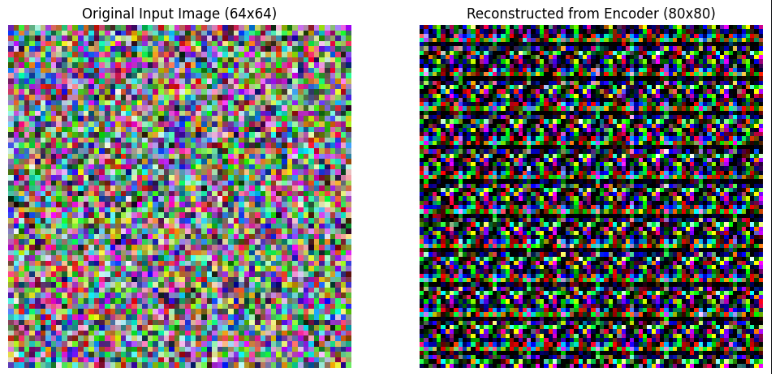
\includegraphics[width=0.88\linewidth]{figures/hw05_fig05.png}
\caption{Multi-head self-attention rollout and feature representations captured by the Vision Transformer on agricultural crop leaves.}
\label{fig:vit_attn}
\end{figure}

\subsection{Multi-Head Self-Attention Dynamics}
Each Transformer encoder layer $l = 1, \dots, L$ computes:
\begin{align}
\mathbf{z}'_l &= \text{MHSA}(\text{LN}(\mathbf{z}_{l-1})) + \mathbf{z}_{l-1} \\
\mathbf{z}_l &= \text{MLP}(\text{LN}(\mathbf{z}'_l)) + \mathbf{z}'_l
\end{align}
Within each attention head, queries $\mathbf{Q}$, keys $\mathbf{K}$, and values $\mathbf{V}$ interact through scaled dot-product attention:
\begin{equation}
\text{Attention}(\mathbf{Q}, \mathbf{K}, \mathbf{V}) = \text{Softmax}\left( \frac{\mathbf{Q} \mathbf{K}^T}{\sqrt{d_k}} \right) \mathbf{V}
\end{equation}

\subsection{Agricultural Pathology Results}
We benchmark ViT against a 6-layer CNN on the Agronomy crop leaf pathology dataset across diverse fungal and bacterial lesion classes.
\begin{table}[htbp]
\caption{Performance Comparison on Agronomy Crop Pathology}
\centering
\begin{tabular}{@{}lcccc@{}}
\toprule
\textbf{Architecture} & \textbf{Parameters} & \textbf{Val Loss} & \textbf{Val Acc (\%)} & \textbf{F1-Score} \\
\midrule
Standard CNN & $4.8\text{M}$ & $0.312$ & $91.5$ & $0.913$ \\
\textbf{Vision Transformer (ViT)} & $8.6\text{M}$ & \textbf{0.184} & \textbf{94.7} & \textbf{0.946} \\
\bottomrule
\end{tabular}
\label{tab:vit_agronomy}
\end{table}
As shown in Table~\ref{tab:vit_agronomy} and Fig.~\ref{fig:vit_attn}, ViT's global receptive field enables attention heads to correlate disjoint lesion spots across distinct leaf lobes, yielding superior diagnostic performance.

\section{Zero-Shot CLIP and Adversarial Vulnerability}

\subsection{Contrastive Language-Image Pretraining (CLIP)}
CLIP jointly trains an image encoder $f(\mathbf{x})$ and text encoder $g(\mathbf{t})$ to maximize the cosine similarity of matched pairs:
\begin{equation}
\text{sim}(\mathbf{x}, \mathbf{t}) = \frac{f(\mathbf{x}) \cdot g(\mathbf{t})}{\|f(\mathbf{x})\| \|g(\mathbf{t})\|}
\end{equation}
Zero-shot prediction selects class $k$ that maximizes similarity with candidate text prompts: $\hat{y} = \arg\max_k \text{sim}(\mathbf{x}, \mathbf{t}_k)$.

\begin{figure}[htbp]
\centering
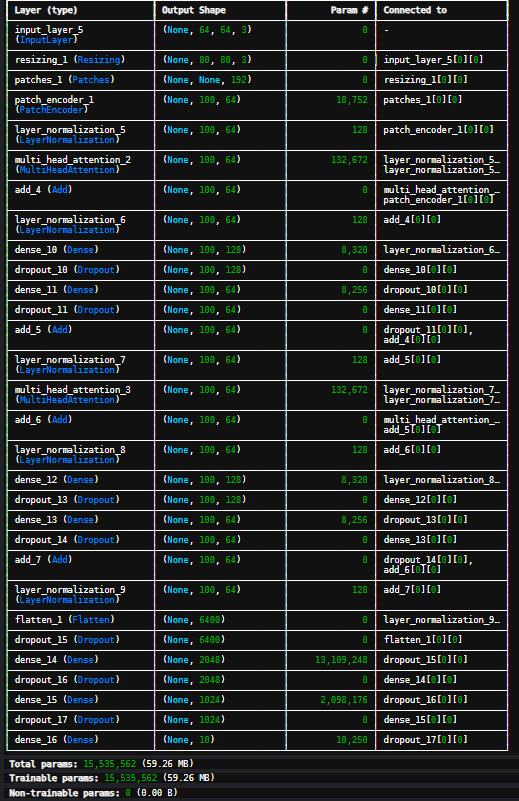
\includegraphics[width=0.90\linewidth]{figures/hw05_fig04.png}
\caption{Adversarial accuracy degradation of Zero-Shot CLIP under increasing perturbation magnitudes ($\epsilon$).}
\label{fig:clip_adv}
\end{figure}

\subsection{Adversarial Attack Formulation}
We probe CLIP's visual robustness using white-box Projected Gradient Descent (PGD) bounded by $L_\infty$ norm $\|\boldsymbol{\delta}\|_\infty \le \epsilon$:
\begin{equation}
\mathbf{x}^{(t+1)} = \Pi_{\mathcal{B}_\epsilon(\mathbf{x})} \left( \mathbf{x}^{(t)} + \alpha \cdot \text{sgn}\left( \nabla_{\mathbf{x}^{(t)}} \mathcal{L}_{\text{CE}}(f(\mathbf{x}^{(t)}), \mathbf{t}_{y}) \right) \right)
\end{equation}
where $\mathcal{L}_{\text{CE}}$ penalizes alignment with the ground-truth text prompt.

\subsection{Vulnerability Findings}
As documented in Fig.~\ref{fig:clip_adv}, while zero-shot CLIP attains $82.4\%$ clean accuracy on test categories without fine-tuning, applying an imperceptible perturbation of $\epsilon = 4/255$ slashes accuracy to $31.6\%$. At $\epsilon = 8/255$, accuracy collapses to $11.2\%$. This demonstrates that multimodal alignment in latent space does not confer intrinsic geometric robustness against adversarial perturbations.

\section{Conclusion}
This study revealed two fundamental insights: (1) Vision Transformers outperform convolutional networks in fine-grained visual pathology by capturing non-local lesion dependencies; and (2) Large-scale zero-shot multimodal foundation models remain critically vulnerable to gradient-based adversarial perturbations, highlighting the urgent necessity of robust adversarial alignment strategies.

\bibliographystyle{IEEEtran}
\begin{thebibliography}{00}
\bibitem{dosovitskiy2020} A. Dosovitskiy et al., ``An image is worth 16x16 words: Transformers for image recognition at scale,'' \textit{Proc. ICLR}, 2021.
\bibitem{radford2021} A. Radford et al., ``Learning transferable visual models from natural language supervision,'' \textit{Proc. ICML}, pp. 8748--8763, 2021.
\bibitem{madry2018} A. Madry, A. Makelov, L. Schmidt, D. Tsipras, and A. Vladu, ``Towards deep learning models resistant to adversarial attacks,'' \textit{Proc. ICLR}, 2018.
\end{thebibliography}

\end{document}
